\section{Decentralising the access to personal data with Solid}
\label{sec:sota_solid}

As attested in Section \ref{sec:def_decentralised_env}, current efforts are underway to decentralise today's Web. By decoupling data from applications, Web users will have their data stored in an environment they can control and can choose what data they want to make publicly accessible or accessible only to certain users while using their application of choice to manage said data.
This represents a significant paradigm shift regarding users' current online experience -- instead of being locked away in Big Tech companies' storage servers, data can be stored on individual personal datastores maintained by a provider chosen by the user or hosted by the user itself on its private server.
In this context, the Solid project \citep{sambra_solid_2016,mansour_demonstration_2016} has been gaining prominence as it relies on Web standards to achieve this degree of decentralisation -- its ultimate goal is to give Web users a personal datastore, i.e., a Pod, per user, with a granular access control system managed by the user, which they can use to select which people and/or applications have access to the resources stored on their Pod.
As such, with Solid, applications and the companies behind them do not store the (personal) data of their users, acting only as interfaces that can read, write or append data to/from Pods.
Such an ecosystem \textit{``fosters innovation and competition through separate markets for data and applications''} \citep{verborgh_paradigm_2017}, while allowing Web users to exert a degree of control over their data that is currently impossible to wield.

In particular, the Solid protocol \citep{capadisli_solid_2022} describes how servers and apps should behave by relying on the following Web standards:

\begin{itemize}
    \item HTTP \citep{fielding_http_2022} -- The Hypertext Transfer Protocol describes an architecture and semantics for \textit{``distributed, collaborative, hypertext information systems''} to share data.
    \item RDF \citep{cyganiak_rdf_2014} -- The Resource Description Framework defines a data model to represent information in the Web, including a schema \citep{brickley_rdf_2014} and serialization syntaxes for storing and exchanging RDF such as Turtle \citep{prudhommeaux_rdf_2014} and JSON-LD \citep{gregg_kellogg_json-ld_2020}.
    \item LDP \citep{speicher_linked_2015} -- The Linked Data Platform specification expresses how to use \textit{``HTTP for accessing, updating, creating and deleting resources from servers that expose their resources as Linked Data''}.
    \item SPARQL \citep{harris_sparql_2013} -- The SPARQL language can be used to query RDF databases. %Solid also uses a subset of SPARQL UPDATE through HTTP PATCH queries.
    \item WebID-TLS \citep{story_webid-tls_2014} -- A protocol that uses WebIDs to authenticate users on the Web.
    \item OIDC \citep{sakimura_openid_2014} -- The OpenID Connect standard is an authentication protocol to assert the users' identity. 
\end{itemize}

Moreover, Table \ref{tab:definitions} provides an overview of Solid-related concepts, their definitions and corresponding classes and properties already modelled in Solid-related vocabularies.
The authentication and authorisation protocols compose Solid's two main building blocks -- an up-to-date list of Solid specifications, including technical reports for both aforementioned building blocks, is maintained by the Solid Community Group at \url{https://solidproject.org/TR/}.
Authentication is a necessary feature to identify users when they want to log into their Pod and/or when they want to use an app to perform a certain action over resources stored in their Pod.
Thus, Solid's authentication protocol uses Solid's WebID specification to identify agents through URIs, as specified in Table \ref{tab:definitions}, which when dereferenced return a WebID profile document that should include information regarding the identity provider chosen by the Solid user and the Pod storage location and may include information regarding an available inbox where users and applications can leave messages to the user \citep{balseiro_solid_2022}.
In addition, to verify the identity of agents, the Solid Protocol recommends the usage of the Solid OIDC protocol\footnote{A Solid-OIDC Primer \citep{morgan_oidcprimer_2022} is also being developed to provide additional knowledge on Solid OIDC's authentication flows.} \citep{coburn_oidc_2022}, however additional authentication methods, such as the previously mentioned WebID-TLS, can also be implemented.

The authorisation protocol specifies mechanisms used by Solid servers to reply to requests of particular users or apps to have access to certain resources, containers of resources or even to the whole Pod.
Furthermore, the Solid protocol states that a Solid server \textit{``MUST conform to either or both Web Access Control (WAC) and Access Control Policy (ACP) specifications''} in order for it to be a compliant Solid server.
Specific authorisation use cases and requirements are documented by the \cite{solid_editorial_team_use_2023} and further details on the authorisation methods will be given in Section \ref{sec:sota_solid_access_control}.
In addition to the authorisation specifications, there is a third protocol being developed to ensure data interoperability and (re)usability across Pod providers, agents and applications -- the Solid Application Interoperability (SAI) specification \citep{bingham_interop_2023}.

\begin{landscape}
\begin{table}[ht]
\caption{Overview of Solid-related concepts, their definitions and related terms modelled on Solid specifications.}
\label{tab:definitions}
\begin{tabular}{c||l|c}
\textbf{Concept} & \textbf{Definition} & \textbf{Solid vocabularies} \\ \hline\hline
Pod & A personal datastore that conforms to the Solid protocol & \texttt{pim:Storage} \\ \hline
Resource & \begin{tabular}[c]{@{}l@{}}Target asset stored in a Pod identified by a URI. Container resources can contain \\ other resources including containers\end{tabular} & \begin{tabular}[c]{@{}c@{}}\texttt{acl:accessTo}, \\ \texttt{acp:target} \end{tabular} \\ \hline
Inbox & Container resource for messages sent to an agent & \begin{tabular}[c]{@{}c@{}}\texttt{ldp:inbox}, \\ \texttt{interop:hasInbox}\end{tabular} \\ \hline
Server & Server capable of hosting resources and responding to resource requests & \\ \hline
App & An application that reads and writes data to Pods & \begin{tabular}[c]{@{}c@{}}\texttt{interop:Application}, \\ \texttt{acp:client}, \texttt{acl:origin}\end{tabular} \\ \hline
Agent & A person, social or virtual entity identified by a URI & \begin{tabular}[c]{@{}c@{}}\texttt{interop:Agent}, \\\texttt{acl:agent}, \texttt{acp:agent}\end{tabular} \\ \hline
\begin{tabular}[c]{@{}c@{}}Pod \\ Owner\end{tabular} & Agent that has control over all resources in a Pod including access control resources & \begin{tabular}[c]{@{}c@{}}\texttt{solid:owner}, \\ \texttt{acp:owner}\end{tabular} \\ \hline
WebID & \begin{tabular}[c]{@{}l@{}}URI that acts as a primary identifier for agents, which, when dereferenced, resolves \\ to an identity profile document (WebID profile)\end{tabular} & \\ \hline
\begin{tabular}[c]{@{}c@{}}Identity \\ Provider\end{tabular} & Entity implementing the identity service capable of authenticating a WebID & \begin{tabular}[c]{@{}c@{}}\texttt{solid:oidcIssuer}, \\ \texttt{acp:issuer}\end{tabular} \\ \hline
\begin{tabular}[c]{@{}c@{}}Pod \\ Provider\end{tabular} & Entity providing the storage space and maintaining the server implementation & \\ \hline
Policy & Conditions for accessing the Pod and its resources & \texttt{acp:Policy} \\ \hline
Registry & Records where agents can store and find different types of data for different purposes & \texttt{interop:Registry}
\end{tabular}
\end{table}
\end{landscape}

\subsection{Access control and interoperability in Solid}
\label{sec:sota_solid_access_control}

As discussed in the previous Section, there are two distinct access control methods being specified in the Solid ecosystem -- both use URIs to identify resources and users, while WAC \citep{capadisli_wac_2022} relies on ACLs and ACP \citep{bosquet_acp_2022} on Access Control Resources (ACRs) to specify who is authorised or refused access and access grants to represent the final authorisation decision.
While server providers can implement only one of the authorisation protocols, Solid applications can not do the same or else they will not work with server providers that use a distinct protocol from the one they choose to implement.
Listings \ref{list:wac} and \ref{list:acp} provide examples of both types of access control statements.
As is visible by the examples, both solutions do not have the depth to deal with the users \textit{`Right to be Informed'} (GDPR's Article 13 and 14), since these models do not contain the terms to specify the purpose for accessing data on Pods, the personal data categories being consulted, used legal basis or even information on the identity of application developers.

\begin{listing}[h]
\caption{WAC authorisation that makes a WebID profile, \url{https://solidweb.me/besteves4/profile/card}, readable by any agent.}
\label{list:wac}
\begin{minted}{turtle}
<#public> a acl:Authorization ;
    acl:agentClass foaf:Agent ;
    acl:accessTo <https://solidweb.me/besteves4/profile/card> ;
    acl:mode acl:Read .
\end{minted}
\end{listing}

\begin{listing}[h]
\caption{ACP authorisation that makes a WebID profile, \url{https://solidweb.me/besteves4/profile/card}, issued by \url{https://solidweb.me/}, readable by any agent using any application.}
\label{list:acp}
\begin{minted}{turtle}
<#public> a acp:AccessGrant ;
    acp:grant acl:Read ;
    acp:context [
        acp:agent acp:PublicAgent ;
        acp:target <https://solidweb.me/besteves4/profile/card> ;
        acp:client acp:PublicClient ;
        acp:issuer <https://solidweb.me/> ] .
\end{minted}
\end{listing}

Moreover, these access protocols were deemed not enough to ensure the interoperability of agents, data and applications and, as such, an interoperability specification is being developed to describe the implementation of agent, data and access registries, to track user interactions with other agents, to keep records of where data is being stored and to manage access grants given to other agents \citep{bingham_interop_2023}.
Listing \ref{list:interop_registryset} provides an example of a registry set which should only be readable by the Pod owner and Listing \ref{list:interop_authz_registry} an example of an authorisation registry, which contains an \texttt{AccessAuthorization} for the \texttt{projectron} app which requires data with a particular shape\footnote{SAI assumes the use of ACL access modes which are still not approved, e.g. \texttt{acl:Create}, \texttt{acl:Update}, \texttt{acl:Delete}, and are under discussion on the Solid CG authorisation panel (see issue at \url{https://github.com/solid/authorization-panel/issues/253}).}. While SAI is a step forward in Solid towards having a more transparent ecosystem, it is still in the early stages of development and as such it is still not clear how this specification will fit in with the existing access control protocols or how it is going to be implemented/enforced.
In addition, as is illustrated by Listing \ref{list:interop_authz_registry}, SAI does not entirely fulfil GDPR requirements, e.g., it does not provide transparency regarding the purpose for access or which type of data is being accessed nor does it provide information regarding the identity of the entities that develop/provide the apps.

\begin{listing}[h]
\caption{Registry set, established according to the SAI specification, that stores private information regarding storage location of registries of \url{https://solidweb.me/besteves4/}.}
\label{list:interop_registryset}
\begin{minted}{turtle}
PREFIX beatriz-registry: <https://solidweb.me/besteves4/registry/>
PREFIX beatrizWork-registry: <https://solidweb.me/besteves4-work/registry/>

beatriz-registry: a interop:RegistrySet ;
  interop:hasAgentRegistry beatriz-registry:agents ;
  interop:hasAuthorizationRegistry beatriz-registry:authz ;
  interop:hasDataRegistry beatriz-registry:data , beatrizWork-registry:data .
\end{minted}
\end{listing}

\begin{listing}[p]
\caption{Authorisation registry of \url{https://solidweb.me/besteves4/}.}
\label{list:interop_authz_registry}
\begin{minted}{turtle}
PREFIX beatriz-authz: <https://solidweb.me/besteves4/registry/authz/>
PREFIX projectron: <https://projectron.app/>
PREFIX projectron-shapetrees: <https://projectron.app/shapetrees/>

beatriz-registry:authz a interop:AuthorizationRegistry;
    interop:hasAccessAuthorization beatriz-authz:projectron .

beatriz-authz:projectron a interop:AccessAuthorization ;
    interop:grantedBy <https://solidweb.me/besteves4/profile/card#me> ;
    interop:grantedWith <https://authz.agent/id> ;
    interop:grantedAt "2023-07-31T11:53:01Z"^^xsd:dateTime ;
    interop:grantee projectron:id ;
    interop:hasAccessNeedGroup projectron:need-group ;
    interop:hasDataAuthorization beatriz-authz:54a1b6a0 .

projectron:need-group a interop:AccessNeedGroup ;
    interop:accessNecessity interop:accessRequired ;
    interop:accessScenario interop:PersonalAccess ;
    interop:authenticatesAs interop:SocialAgent ;
    interop:hasAccessDescriptionSet projectron:access-en ;
    interop:hasAccessNeed projectron:need-project .

projectron:need-project a interop:AccessNeed ;
    interop:registeredShapeTree projectron-shapetrees:ProjectTree ;
    interop:accessNecessity interop:accessRequired ;
    interop:accessMode acl:Read, acl:Create ;
    interop:creatorAccessMode acl:Update, acl:Delete .

beatriz-authz:54a1b6a0 a interop:DataAuthorization ;
    interop:grantee projectron:id ;
    interop:registeredShapeTree projectron-shapetrees:ProjectTree ;
    interop:accessMode acl:Read, acl:Create ;
    interop:creatorAccessMode acl:Update, acl:Delete ;
    interop:scopeOfAuthorization interop:All ;
    interop:satisfiesAccessNeed projectron:need-project .
\end{minted}
\end{listing}

Furthermore, the idea of having registries of data and applications is also compatible with the graph-centric interpretation of a Pod debated by \cite{dedecker_whats_2022}. Certain apps might require the presence of particular data stored in a particular container -- this will cause an interoperability problem as it is something that cannot be standardised across the ecosystem for all apps.
With a graph-centric approach, \textit{`each Solid pod is a hybrid, contextualized knowledge graph, wherein ``hybrid'' indicates first-class support for both documents and RDF statements, and ``contextualized'' the ability to associate each of its individual documents and statements with metadata such as policies, provenance, and trust'}.
With such metadata, including context and provenance metadata, distinct views of the Pod can be rendered as required by different applications or agents.
Moreover, data request policies can simply be appended to the \textit{`Pod as a Graph'}, without the need to have it hardcoded in the app, and can be viewed by users using graphic-centric Solid apps.

\subsection{Solid and data protection}
\label{sec:sota_solid_data_protection}

Only recently has the debate on data protection reached the concerns of Solid's developers, mainly with regard to issues of control and privacy of personal data.
In addition, beyond the access control mechanisms discussed in the previous Section, there are also researchers starting to work on \textit{`usage control'}, a process which has as its main concern the enforcement of the users' policies after the access to the data has already been given \citep{akaichi_semantic_2022,havur_greater_2020}.
As such, in this Section, we describe the existing body of work on data protection and governance aspects of Solid-related technologies, with a particular focus on GDPR-related academic and industrial research.

\paragraph{Exercising of data subject rights} 
\cite{de_mulder_prov4itdata_2021} developed PROV4ITDaTa\footnote{The source code is available at \url{https://github.com/RMLio/prov4itdata-web-app}, under an MIT license (accessed on 14 August 2023).}, a configurable application that facilitates the exercising of the data subject's \textit{`right to data portability'}, using open sources resources such as RML.io\footnote{\url{https://rml.io/} (accessed on 14 August 2023)} \citep{dimou_rml_2014} -- to access and generate interoperable Linked Data datasets using the Schema.org or DCAT vocabularies, Solid -- to store the datasets, and Comunica\footnote{\url{https://comunica.dev/} (accessed on 14 August 2023)} \citep{taelman_comunica_2018} -- to query the datasets, and promotes transparency by automatically generating and recording provenance metadata using the PROV Ontology standard.
The PDS Interop collaboration \citeyearpar{noauthor_pds_2021}, an effort that started with the goal to make Solid and Nextcloud\footnote{\url{https://nextcloud.com/} (accessed on 20 August 2023)} interoperable, also developed an app, the Solid Migrator App\footnote{The source code is available at \url{https://github.com/pdsinterop/solid-migrator-app}, under an MIT license (accessed on 20 August 2023).}, to assist in the migration of Pod resources to a different Pod, independently of the Pod provider.

\paragraph{GDPR principles}
\cite{pandit_making_2023} describes Solid as a \textit{`cloud technology'}, according to ISO standards, provides a theoretical discussion on how GDPR principles apply to Solid and suggests how to extend its specifications to deal with such requirements.
\cite{esposito_assessing_2023} also provide a theoretical analysis of technical security and privacy measures to assist Solid developers in complying with the GDPR -- a mapping of Solid actors and respective legal roles is provided for accountability, as well as security measures to ensure data confidentiality and minimisation and protocols to safeguard the data subjects' rights to be notified, to object and to not be a target of automated decision-making.
\cite{van_damme_towards_2022} present a qualitative analysis of a series of plenary sessions with academia, governments, citizens and industry regarding the adoption of decentralised personal datastore technologies. The main challenges that were identified are related to social, technical, legal and ecosystem issues, which need to be considered for the \textit{``development of an interdisciplinary research agenda''}. In terms of legal challenges, the core aspects that were discussed are related to control, portability, compliance, accountability, delegation of consent and the usage of other legal bases such as legitimate interests. The role of intermediates, promoted by the DGA, was also discussed. % Use cases related to mobility, media, health, finance and administration were also discussed.
Digita\footnote{\url{https://www.digita.ai/} (accessed on 15 August 2023)}, a Belgian startup that offers Solid-based identity and storage solutions, published a research report reflecting on accountability aspects related to the implementation of Solid products, mainly regarding the lawfulness of data usage and transfer to recipients, particularly based on consent, and the specificity and compatibility of purposes \citep{de_bot_data_2021}.
\cite{bailly_prototyping_2023} propose to use the SAI and DPV vocabularies to specify access and usage control policies, respectively, and provide a prototype User Interface (UI) for users to consent to data requests\footnote{The source code is available at \url{https://github.com/HBailly/solid-auth-ui/}, under a GNU General Public License v3.0 (accessed on 15 August 2023).}, which the authors found to have a low score in terms of usability.
% athumi (flemish data utility company) not discussed, find paper?

\paragraph{Domain-specific use cases}
Several health-related use cases have been developed by the Solid research community.
Among them, TIDAL\footnote{The source code is available at \url{https://github.com/sunchang0124/TIDAL}, under an MIT license (accessed on 15 August 2023).} (ciTIzen-centric DAta pLatform), a Solid-powered application, has been developed by \cite{sun_citizen-centric_2023} for healthcare researchers to request consent from citizens to use their data for health-related research. DPV is used to limit the purpose for which the data can be used, DPV-PD and other health-related vocabularies to restrict the categories of personal data and privacy-preserving data analysis algorithms to preserve data confidentiality.
Janeiro Digital\footnote{\url{https://www.janeirodigital.com/} (accessed on 15 August 2023)} \citeyearpar{noauthor_janeiro_nodate} is working with the United Kingdom's National Health Service (NHS) to manage and use patient data from several systems, providing patients with individual Solid Pods and giving healthcare professionals access to data through the Solid protocol.
\cite{ammar_personal_2020,ammar_using_2021} discuss the implementation of a \textit{``Personal Health Library''} using Solid \textit{``to deliver tailored push notifications to support behavior change related to chronic disease self-care''} based on sensor readings and other information.
In addition, they are developing an app to allow users to decide what data should be stored in the Pod, and who should have access to it, and to share their data with other research initiatives.

In addition to the work of \cite{de_bot_data_2021}, \cite{chugunov_streamlining_2020} also focus on government-related use cases. In this work, a Solid app for Flemish citizens, that allows them to share data with government administrations and to reuse said data in different contexts, is described to increase the accuracy of personal data which is difficult to keep updated, e.g., telephone numbers or email addresses, and to allow data portability.
\citeauthor{wang_enhancing_2020}'s thesis also discusses the usage of Solid to enhance governmental services, including provisions to improve the access and rectification rights exercised in this context, including a use case scenario of applying to a social house and dealing with the subsequent changes to the address. 

Karamel\footnote{\url{https://karamel.career/} (accessed on 20 August 2023)} also partnered with Digita to create a human resources platform for applicants and recruiters to find new jobs \citep{verstraete_solid_2022} -- users can manage data stored in Solid Pods through an app that allows applicants to revoke access and to request to be forgotten by recruiters.

\cite{toth_preserving_2022} developed a prototype architecture for the domain of hospitality where users can use Solid applications to book/manage accommodations and edit personal information. This proof of concept\footnote{The source code is available at \url{https://github.com/gergelyth/solid-hotel}, under an MIT license (accessed on 21 August 2023).} allows its users to request deletion and rectification of data and of copies of said data.

\cite{van_de_wynckel_solidbased_2022} are researching the usage of Solid to develop transparent indoor positioning systems that store individual and sensor data in Solid Pods in an interoperable format. In addition, they developed an app that reads the user’s personal position, orientation and velocity from the Pod and displays them along with additional information\footnote{The source code is available at \url{https://github.com/OpenHPS/ipin2022-solid/} (accessed on 23 August 2023).}.

The described solutions can be compared through Figure \ref{fig:solid_sota}.
Each solution was analysed in terms of whether it assists in the exercising of data subject rights or in the implementation of a certain GDPR principle, as well as the type of solution developed by the authors of the paper.
Works describing Solid apps are marked with a \textbf{black} shape, identity provider solutions with a \textbf{\textcolor{orange}{orange}} shape, Pod provider solutions with a \textbf{\textcolor{blue}{blue}} shape and theoretical work with a \textbf{\textcolor{red}{red}} shape.
In addition, works marked with a $\medcircle$ discuss a government-related use case, $\medtriangleup$ a health-related use case, $\meddiamond$ a hospitality-related use case, \faStarO\space a location-related use case, $\medsquare$ a human resources-related use case and \textbf{X} represents work without a particular domain-related use case.
As illustrated by the Figure, most works concentrate on fulfilling one or more GDPR principles, with a strong focus on the \textit{`lawfulness, fairness and transparency'} principle.
Distinct works were also found to tackle the right to data portability, withdrawal of consent and rectification, while no specific work was found on the right to restrict the processing of personal data. 

\begin{figure}
\caption[Comparison of existing work on Solid and data protection topics.]{Comparison of existing work on Solid and data protection topics. Each work was analysed in terms of whether it assists in the exercising of data subject rights or in the implementation of a certain GDPR principle, as well as the type of solution they developed -- works describing Solid apps are marked with a \textbf{black} shape, identity provider solutions with a \textbf{\textcolor{orange}{orange}} shape, Pod provider solutions with a \textbf{\textcolor{blue}{blue}} shape and theoretical work with a \textbf{\textcolor{red}{red}} shape. In addition, works marked with a $\medcircle$ discuss a government-related use case, $\medtriangleup$ a health-related use case, $\meddiamond$ a hospitality-related use case, \faStarO\space a location-related use case, $\medsquare$ a human resources-related use case and \textbf{X} represents work without a particular domain-related use case.}
\label{fig:solid_sota}
\centering
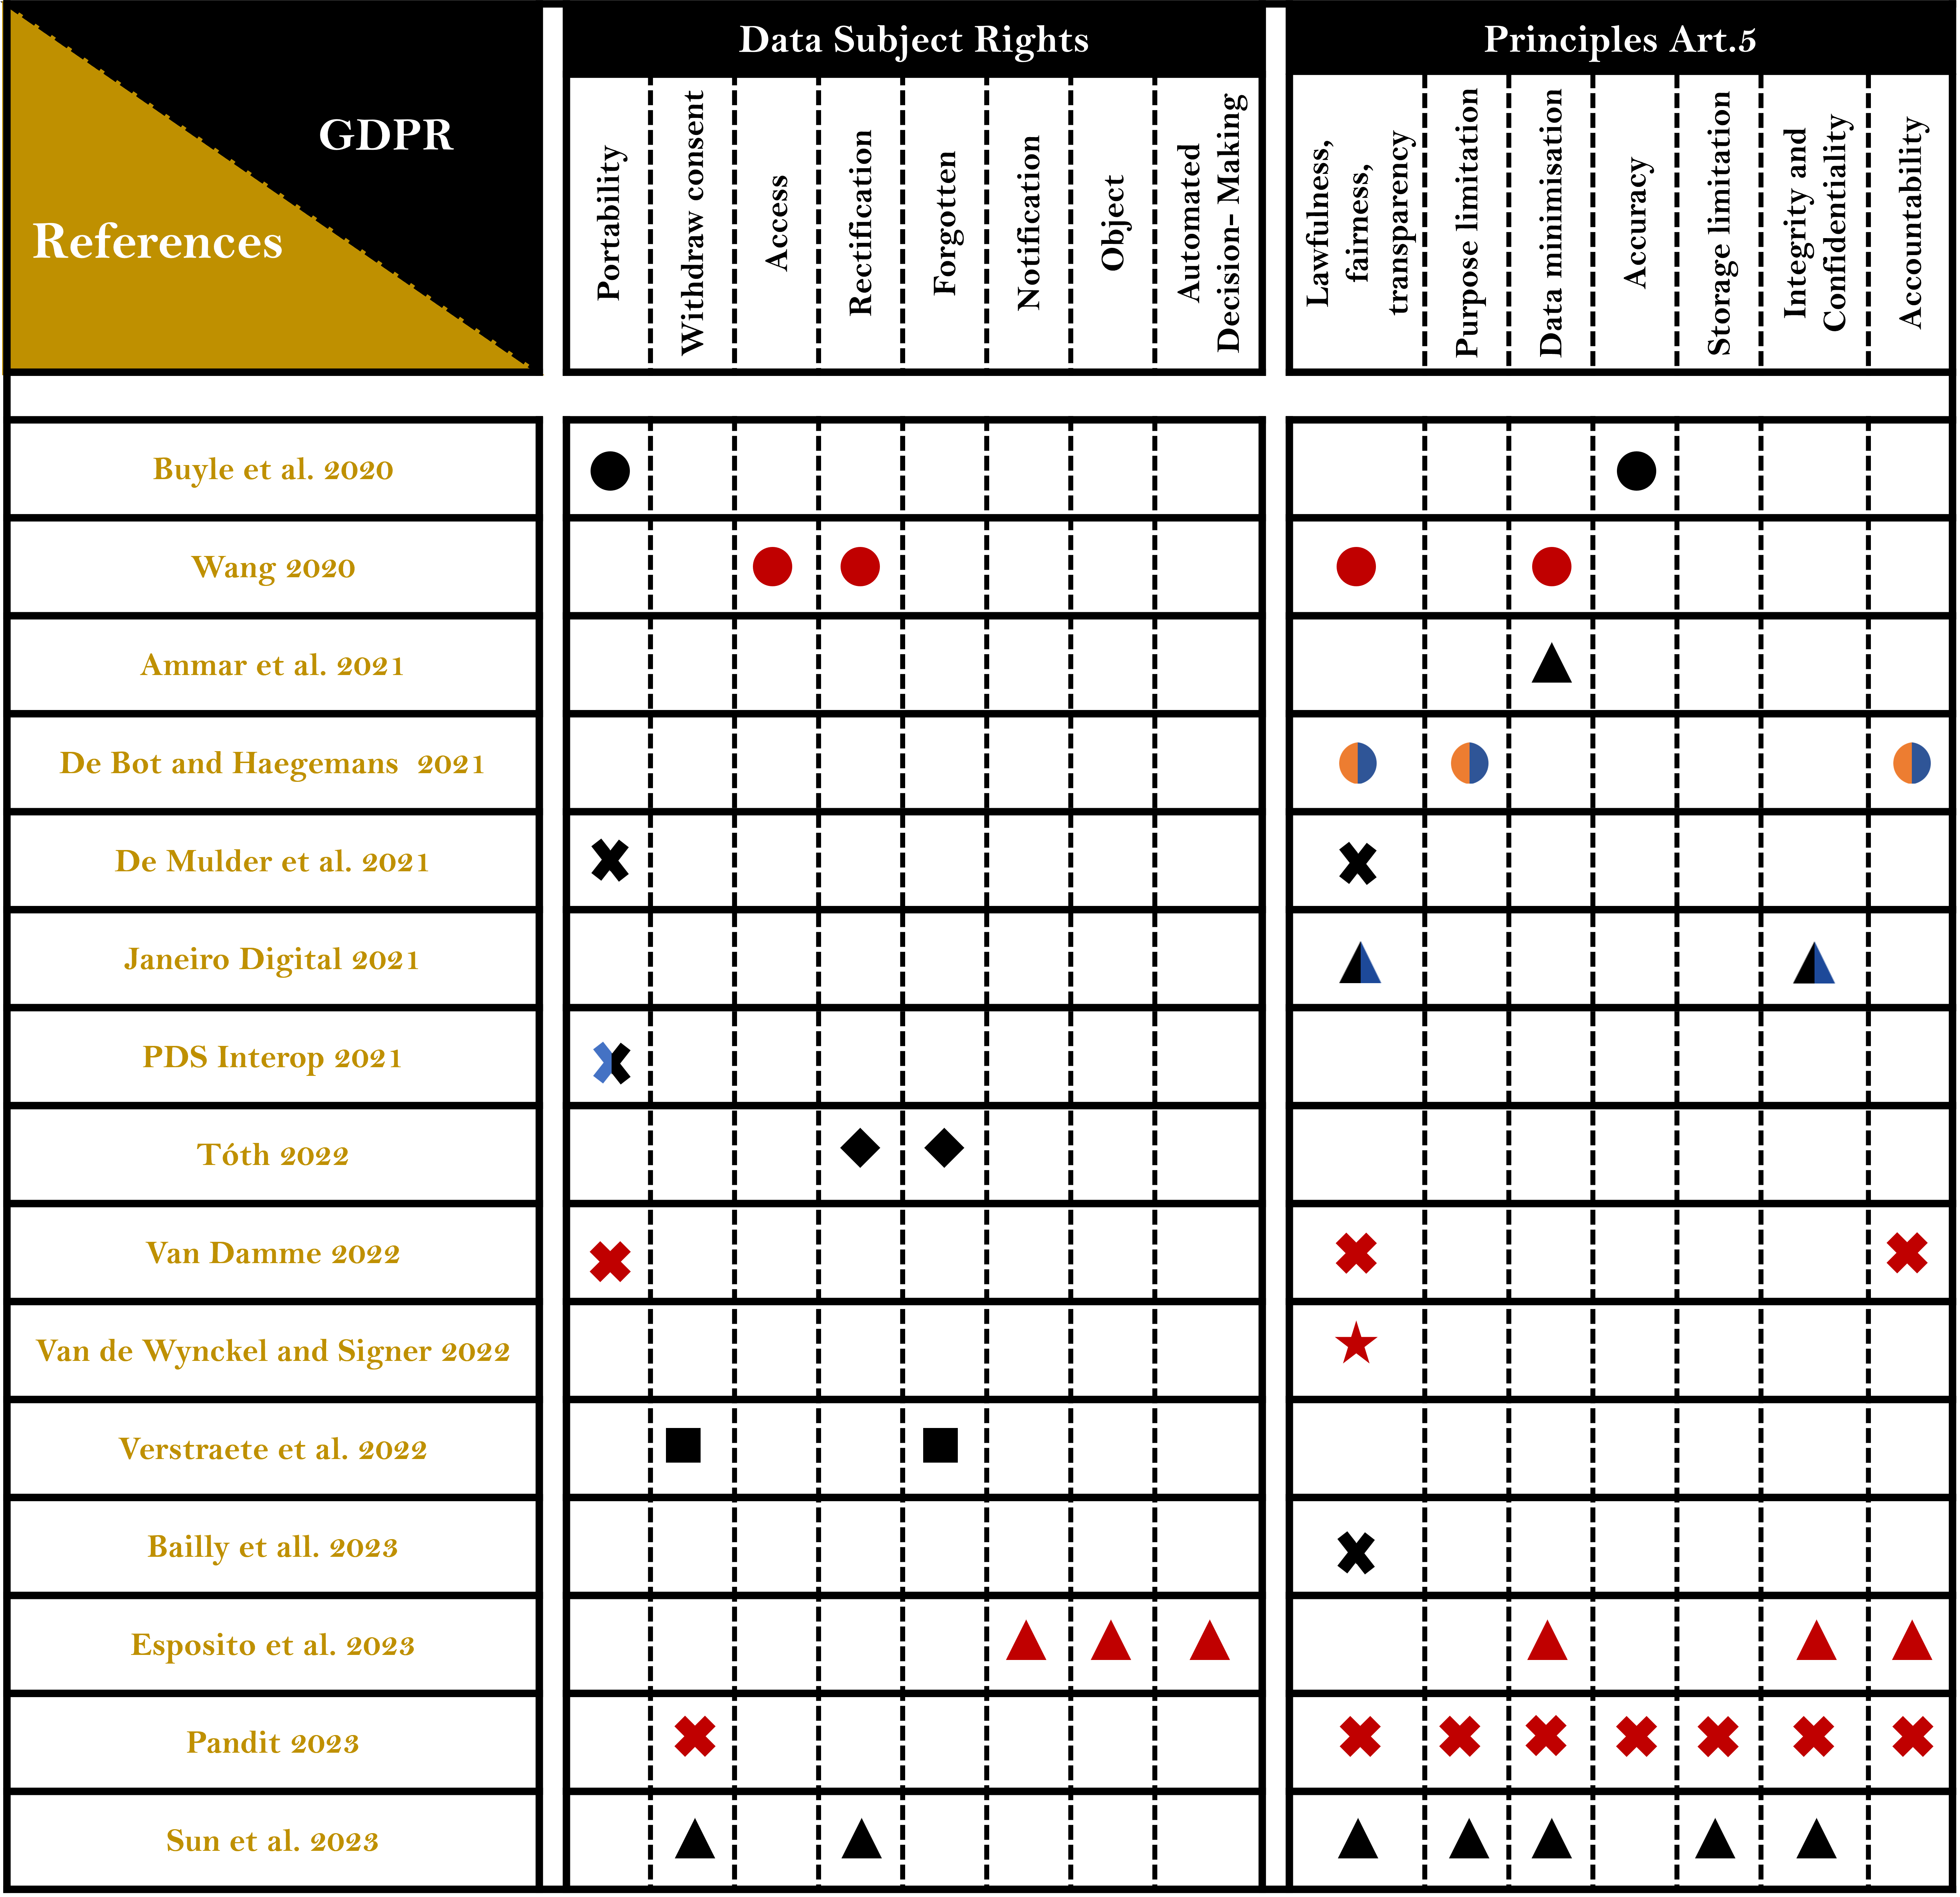
\includegraphics[width=\textwidth]{figures/chapter-2/solid-sota.png}
\end{figure}

%Inrupt\footnote{\url{https://www.inrupt.com/} (accessed on 20 August 2023)}, an enterprise co-founded by Sir Tim Berners-Lee to create Solid products and to help advance and maintain the Solid protocol, is working with the BBC\footnote{\url{https://www.bbc.com/} (accessed on 20 August 2023)} \citep{kuesel_bbc_2022} and with NatWest\footnote{\url{https://www.natwest.com/} (accessed on 20 August 2023)} \citep{olivo_solid_2020} to provide Solid apps to these companies that offer personalised services to their costumers, e.g., recommend a new program to watch or to open a new bank account, respectively.

%\cite{hochstenbach_rdf_2023} are developing RDF Surfaces\footnote{\url{https://w3c-cg.github.io/rdfsurfaces/}}, a Notation3 language which intends to bring first-order logic to the Semantic Web and therefore can be used to \textit{``provide enforcement of data policies using logic-based rules''}.

\subsection{Other decentralised technologies}
\label{sec:sota_other_technologies}

In addition to Solid and its stack of technologies, there is a set of tools and resources that support decentralisation and are either being discussed or should be discussed to be included in the Solid ecosystem.
We briefly present them in this Section as they should be considered in future research in this area.

\paragraph{Decentralised Identity}
The Decentralized identifiers (DIDs) data model is a recent W3C Recommendation that enables \textit{``individuals and organizations to generate their own identifiers using systems they trust''} \citep{sporny_decentralized_2022}\footnote{A DID Solid method specification is in the early stages of development, with no official implementations being known to date -- available at \url{https://solid.github.io/did-method-solid/} (accessed on 19 August 2023).}.
In contrast with centralised settings, DIDs allow something or someone to be identified by a globally unique identifier which is detached from centralised registries, identity providers, or certificate authorities.
Moreover, DIDs work in a similar fashion to WebIDs -- DIDs are still URIs that can be dereferenced to return a DID document which \textit{``can express cryptographic material, verification methods, or services [...] to prove control of the DID''}.
The European Commission is also promoting the emergence of digital identity wallets for EU citizens, residents and businesses to identify themselves, both online and offline, and to exchange certain types of personal identification data such as birth certificates or driving licenses.
In this context, the electronic IDentification, Authentication and trust Services (eIDAS) regulation \citeyearpar{noauthor_regulation_2014}, and its amendment \citeyearpar{noauthor_eidas2_2021}, puts forward \textit{``rules for trust services''} and \textit{``a legal framework for electronic signatures, electronic seals, electronic time stamps, electronic documents, electronic registered delivery services and certificate services for website authentication''}, while the 2021 amendment explicitly adds \textit{``conditions for the issuing of European Digital Identity Wallets''} and additional considerations derived from the GDPR.

\paragraph{Verifiable Credentials}
W3C's Verifiable Credentials (VCs) data model specification describes \textit{``a standard way to express credentials on the Web in a way that is cryptographically secure, privacy-respecting, and machine-verifiable''} \citep{sporny_verifiable_2023}, using technologies such as digital signatures. As in the physical world, VCs can be used to identify data subjects, to provide government-issued documents, e.g., ID cards or passports, or to deliver information on how the credential was created/derived and other constraints such as validity period or conditions for use. An example of a VC, with a DID-identifiable subject, is presented in Listing \ref{list:vc_fromspec}. The usage of VCs is being contemplated in the ACP specification, however, no specific details are provided regarding its implementation/development.

\begin{listing}[htbp]
\caption[Verifiable credential with terms of use, extracted from \cite{sporny_verifiable_2023}.]{Verifiable credential with terms of use where the issuer is prohibiting verifiers from archiving a degree credential, extracted from \cite{sporny_verifiable_2023}, with the credential subject being identified by a DID.}
\label{list:vc_fromspec}
\begin{minted}{json}
{
    "@context": [
        "https://www.w3.org/ns/credentials/v2",
        "https://www.w3.org/ns/credentials/examples/v2"
    ],
    "id": "http://university.example/credentials/3732",
    "type": ["VerifiableCredential", "ExampleDegreeCredential"],
    "issuer": "https://university.example/issuers/14",
    "validFrom": "2010-01-01T19:23:24Z",
    "credentialSubject": {
        "id": "did:example:ebfeb1f712ebc6f1c276e12ec21",
        "degree": {
          "type": "ExampleBachelorDegree",
          "name": "Bachelor of Science and Arts"
        }
    },
    "termsOfUse": [{
        "type": "IssuerPolicy",
        "id": "http://example.com/policies/credential/4",
        "profile": "http://example.com/profiles/credential",
        "prohibition": [{
            "assigner": "https://university.example/issuers/14",
            "assignee": "AllVerifiers",
            "target": "http://university.example/credentials/3732",
            "action": ["Archival"]
        }]
    }] 
}
\end{minted}
\end{listing}

Moreover, \cite{braun_selfverifying_2022,braun_attributebased_2022} have previously published work on using VCs and RDF-star\footnote{RDF-star\citep{arndt_rdfstar_2023} is an under-development W3C specification that \textit{``extends RDF with a convenient way to make statements about other statements''}.} to sign and verify Web resources using a Solid app\footnote{The source code is available at \url{https://github.com/uvdsl/solid-web-ldsig}, under an MIT license (accessed on 19 August 2023).} and on using VCs and Linked Data Notifications (LDNs)\footnote{The W3C LDNs Recommendation \citep{capadisli_linked_2017} is a protocol that describes how servers can send and retrieve RDF-based messages, sent/retrieved by applications.}, extending previous work from \citeauthor{ezike_solidvc_2019}, to request attribute-based access to Solid Pods\footnote{The source code is available at \url{https://github.com/uvdsl/solid-vc-pwa/}, under an MIT license (accessed on 19 August 2023).}.

% TODO: \paragraph{Data Spaces} IDSA + Gaia-X - comparison with solid in enabler paper

% TODO: \paragraph{Interplanetary file system (IPFS)}

% TODO: \paragraph{DTP (Data Transfer Project)}
% A DTP and SoLiD based Service for Multi-Source Semantically-Heterogeneous Personal Data Management